\documentclass[12pt,a4paper]{article}
\usepackage[utf8]{inputenc}
\usepackage[margin=1.5cm]{geometry}
\usepackage{amsmath}
\usepackage{amssymb}
\usepackage{amsthm} 
\usepackage{graphicx}
\usepackage{mathtools}

\DeclarePairedDelimiter{\abs}{\lvert}{\rvert}
\newcommand{\inter}{\begin{matrix}\prod\end{matrix}}
 
\begin{document}
\section*{LEZIONE 17}
\subsection*{Derivazione numerica: instabilità dell'operatore derivata, formule \\
di derivazione approssimata, instabilità e minimizzazione dell'errore}
%PAGINA 1\\%mike
In questa lezione ci occuperemo del calcolo approssimato di derivate a partire da dati discreti (valori campionati di una funzione derivabile), la cosiddetta "derivazione numerica". Consideriamo l'operatore funzionale di derivazione.
%PAGINA 2\\%mike
\begin{equation*}
    D:C^1[a,b]\rightarrow C[a,b],\  \  \  f\longmapsto Df=f'
\end{equation*}
che manda una funzione $f$ derivabile con derivata continua in [a,b] nella sua derivata $f'$.\\ Ricordiamo che si tratta di un operatore \underline{lineare}, infatti 
\begin{equation*}
    (\alpha f+\beta g)'=\alpha f'+\beta g'
\end{equation*}
$\forall f,g$ derivabili e $\alpha,\beta\in\mathbb{R}$.\\A differenza dell'operatore di integrazione $I:C[a,b]\rightarrow\mathbb{R}$,
\begin{equation*}
    f\longmapsto I(f)=\int_a^b f(x)dx
\end{equation*}
che è stabile perché
%PAGINA 3%mike
\begin{equation*}
    |I(f)-I(\tilde{f})|\leq(b-a)dist(f,\tilde{f})
\end{equation*}
e quindi 
\begin{equation*}
    dist(f,\tilde(f))\rightarrow0\Rightarrow|I(f)-I(\tilde{f}|\rightarrow0
\end{equation*}
nel caso della derivazione
\begin{equation*}
    dist(f,\tilde{f})\rightarrow0\nRightarrow dist(f',\tilde{f}')\rightarrow0
\end{equation*}
come si può vedere dal seguente disegno preso dalla lezione 16
\begin{center}
    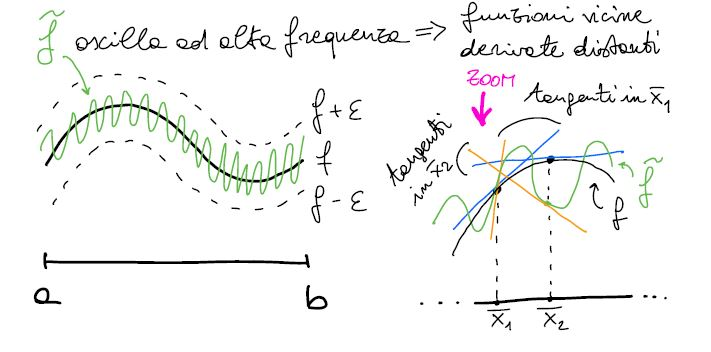
\includegraphics[scale=0.6]{calcolo55.JPG}
\end{center}
%PAGINA 4\\%mike
dove si vede che si può prendere $\tilde{f}$ che oscilla ad alta frequenza intorno ad $f$, in modo tale che $dist(f,\tilde{f})\leq\varepsilon\rightarrow0$ ma $dist(f',\tilde{f}')$ può essere arbitrariamente grand, ovveo l'operatore di derivazione è \underline{POTENZIALMENTE INSTABILE}, concetto che si può parafrasare dicendo "\underline{funzioni} arbitrariamente \underline{vicine possono} avere \underline{derivate} arbitrariamente \underline{distanti}".\\Ovviamente questo dell'oscillazione ad alta frequenza (che ricorda il fenomeno della misura con
%PAGINA 5\\%mike
rumore) è solo un esempio, un altro disegno esplicativo della potenziale instabilità è il seguente 
\begin{center}
    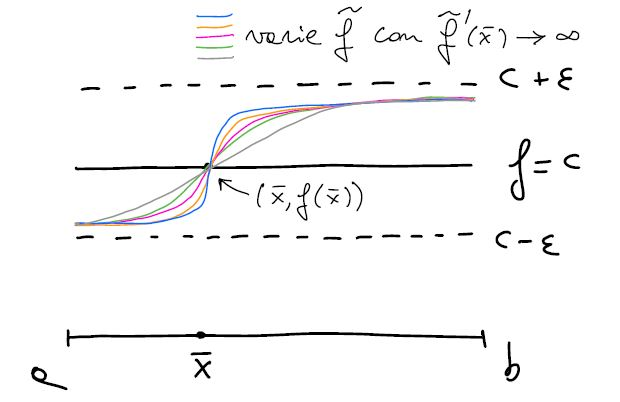
\includegraphics[scale=0.5]{calcolo2.JPG}
\end{center}
in cui in un intorno di una funzione costante (quindi $f'=0$ in [a,b]) compaiono varie funzioni $\tilde{f}$ con derivate via via crescenti in $\bar{x}$.\\
%PAGINA 6\\%mike
Anche qui, possiamo far tendere $\varepsilon\rightarrow0$ e contemporaneamente $|\tilde{f}'(\bar{x})|\rightarrow\infty$ cioè $dist(f,\tilde{f})\rightarrow0$ ma $dist(f',\tilde{f}')\rightarrow\infty$.\\A differenza dell'integrazione, con la derivazione siamo in presenza di un \underline{PROBLEMA} potenzialmente \underline{INSTABILE}, sul quale ci aspettiamo problemi di instabilità "ereditata" da qualsiasi algoritmo di soluzione approssimata.\\Vedremo infatti che anche
%PAGINA 7\\%mike
le più semplici formule di calcolo numerico delle derivate soffrono di perdita di precisione rispetto agli errori nella misura/approssimazione di $f$ e che tale instabilità non può essere completamente eliminata ma solo opportunamente gestita.\\Consideriamo per iniziare il problema del calcolo di $f'$ in un singolo punto $x$ tramite valori di $f$ campionati in un intorno 
\begin{equation*}
    I_r=I_r(x)=[x-r,x+r]
\end{equation*}
assumendo $f\in C^2(I_r)$ e usando
%PAGINA 8\\%mike
il rapporto incrementale destro 
\begin{equation*}
    \delta_+(h)=\frac{f(h+x)-f(x)}{h},\  \  \  0<h\leq r
\end{equation*}
Dalla definizione stessa di derivabilità in $x$ abbiamo che
\begin{equation*}
    \underset{h\rightarrow0}{\lim}\delta_+(h)=f'(x)
\end{equation*}
cioè l'algoritmo di calcolo approssimato della derivata corrispondente al calcolo del rapporto incrementale destro è \underline{convergente} (per questo basterebbe la derivabilità di $f$ in $x$).\\Possiamo però ottenere una
%PAGINA 9\\%mike
stima dell'errore utilizzando la formula di Taylor centrata in $x$ con incremento (passo) $h$
\begin{equation*}
    f(x+h)=f(x)+hf'(x)+\frac{h^2}{2}f''(z)
\end{equation*}
dove $z\in int(x,x+h)$. Allora
\begin{equation*}
    f(x+h)-f(x)=hf'(x)+\frac{h^2}{2}f''(z)
\end{equation*}
cioè
\begin{equation*}
    \delta_+(h)=\frac{f(x+h)-f(x)}{h}=f'(x)+O(h)
\end{equation*}
nel senso che $\exists c>0$ tale che 
\begin{equation*}
    |\delta_+(h)-f'(x)|\leq ch,\  \  \  \  c=\frac{1}{2}\underset{t\in I_r}{max}|f''(t)|\geq\frac{|f''(z)|}{2}
\end{equation*}
%PAGINA 10 \\ %Alessandro 
Ricordiamo la definizione dei principali SIMBOLI ASINTOTICI di variabile $u$ continua ($u\in$1 intervallo) o discreta ($u=\in \mathbb{N}$),cioè sia funzioni che successioni, dove $u \rightarrow \overline{u}$ comprende anche i casi $\overline{u}=\infty$ e $u \rightarrow \overline{u}^{\pm}$, limiti $dx$ e $sin$
\begin{itemize}
    \item simbolo "O-grande": $\alpha(u)=O(\beta(u))$ \\
    per $u \rightarrow \overline{u}$ significa $\exists c > 0$ (indipendente da $u$) tale che $|\alpha(u)| \leq c|\beta(u)| \ \forall u$ in un intorno di $\overline{u}$ 
    \item simbolo "o-piccolo": $\alpha(u)=o(\beta(u))$ \\
    per $u \rightarrow \overline{u}$ significa $\alpha(u) / \beta(u) \rightarrow 0, \ u \rightarrow \overline{u}$
    \item simbolo "$\sim$": $\alpha(u)\sim(\beta(u))$ \\
    per $u \rightarrow \overline{u}$ significa $\alpha(u) / \beta(u) \rightarrow 1, \ u \rightarrow \overline{u}$
\end{itemize}
%PAGINA 11 \\%Alessandro
La convergenza del rapporto incrementale $\delta_+(h)$ a $f'(x)$ è "lenta", essendo l'errore un infinitesimo di ordine 1 in $h$.
\newline
D'altra parte in pratica per presenza di errori (di misura sperimentale o di calcolo di $f$) non avremo (quasi) mai i valori esatti $f(t)$ nei vari $t$ che ci interessano ($t=x$, $t=x+h$) ma solo dei valori approssimati $\Tilde{f}(t)$, di cui supponiamo di saper stimare l'errore
\begin{equation*}
    |f(t) - \tilde{f}(t)| \leq \varepsilon \ \forall t \in I_r
\end{equation*}
%PAGINA 12 \\%Alessandro
Chiamiamo allora $\tilde{\delta}_+(h)$ il rapporto incrementale "perturbato"
\begin{equation*}
    \tilde{\delta}_+(h) = \frac{\tilde{f}(x+h)-\tilde{f}(x)}{h}
\end{equation*}
che è l'unica quantità che siamo effettivamente in grado di calcolare.\\
Possiamo scrivere
\begin{equation*}
    \begin{split}
        & |f'(x)-\tilde{\delta}_+(h)| = |f'(x)-\delta_+(h)+\delta_+(h)-\tilde{\delta}_+(h)| \\
        & \underset{\text{diseg. triangolare}}{\leq} \underset{\text{convergenza}}{|f'(x)-\delta_+(h)|} + \underset{\text{stabilità}}{|\delta_+(h)-\tilde{\delta}_+(h)|}
    \end{split}
\end{equation*}
in cui come al solito separiamo lo studio della convergenza dall'analisi di stabilità.\\
%PAGINA 13 \\%Alessandro
Per quanto riguarda quest'ultima
\begin{equation*}
    \begin{split}
        & |\delta_+(h)-\tilde{\delta}_+(h)| = | \frac{f(x+h) - f(x)}{h} - \frac{\tilde{f}(x+h) - \tilde{f}(x)}{h}| \\
        & = | \frac{f(x+h) - \tilde{f}(x+h)}{h} - \frac{\tilde{f}(x) - f(x)}{h}| \\
        & \underset{\text{diseg. triangolare}}{\leq} \frac{1}{h}|f(x+h) - \tilde{f}(x+h)| + \frac{1}{h}|\tilde{f}(x) - f(x)| \\
        & \leq \frac{1}{h}\varepsilon + \frac{1}{h}\varepsilon = \frac{2\varepsilon}{h}
    \end{split}
\end{equation*}
da cui 
\begin{equation*}
    |\delta_+(h)-\tilde{\delta}_+(h)| \leq ch+\frac{2\varepsilon}{h} = E_+(h)
\end{equation*}
Per $\varepsilon$ fissato (che è l'errore max nel calcolo/campionamento di $f$) si vede che ci sono 2 \underline{esigenze
%PAGINA 14 \\%Alessandro
contrastanti}: da un lato si deve prendere $h$ piccolo per rendere piccolo l'errore legato alla convergenza teorica, cioè l'addendo $ch$ nella stima. Ma allo stesso tempo, per $\varepsilon$ fissato prendere $h \rightarrow 0$ implica che il secondo addenso $\frac{2\varepsilon}{h}\rightarrow \infty$, cioè per $h$ piccolo \underline{l'errore su $f$ viene amplificato}.\\
Questa è l'instabilità "ereditata" dalla potenziale instabilità intrinseca dell'operatore di derivazione (non è vero che
%PAGINA 15 \\ %Alessandro
un errore piccolo su $f$ comporti un errore piccolo su $f'$).\\
\vspace{0.1cm}
\\
Cosa sta succedendo? \\
Per capirlo basta guardare il grafico di $E_+(h)$ in $h$
\begin{center}
    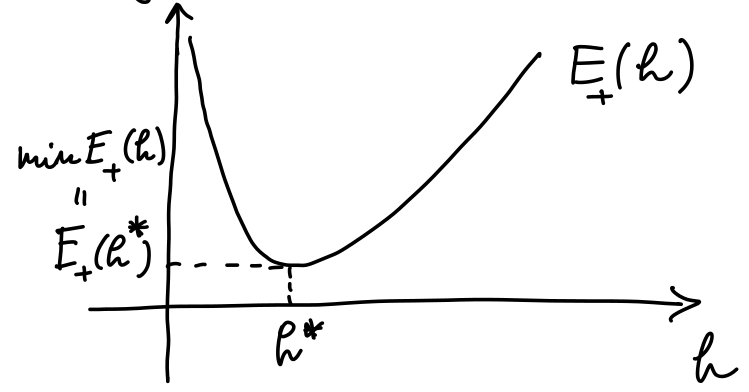
\includegraphics[scale=0.5]{pag15.png}    
\end{center}
la funzione $E_+(h)$ è convessa per $h>0$, non si può prendere $h$ "grande" perché altrimenti domina il termine $ch$, ma
%PAGINA 16\\ %Simone
non si può neppure prendere $h$ troppo piccolo perchè allora domina il termine $\dfrac{2\varepsilon}{h}\to \infty$ per $h\to 0$.\\
Il meglio che si può fare è rpendere il passo $h=h^*$ punto di minimo di $E_+(h)$ (o perlomeno un passo $h$ vicino ad $h^*$ per avere un errore vicino al minimo).\\
Possiamo calcolare il passo ottimale $h^*$ e l'errore minimo $E_+(h)$, trattandosi di una semplice funzione razionale di $h$.\\
%PAGINA 17\\ %Simone
Cerchiamo i punti stazionari di $E(h)$ (dove $E_+'(h)=0$)
\[ \begin{split}
	& E_+'(h)=\left( ch+\frac{2\varepsilon}{h}\right) ' =c-\dfrac{2\varepsilon}{h^2}=0 \\
	& \; \Downarrow \\
	& \; h^2=\dfrac{2\varepsilon}{c}\Rightarrow h^*=h^*(\varepsilon)=\sqrt{\dfrac{2\varepsilon}{c}}
\end{split} \]
Dove con il simbolo $'$ si intende la derivata di $\left( ch+\frac{2\varepsilon}{h}\right) '$ in $h$.\\
Inoltre $E_+''(h)=\dfrac{4\varepsilon}{h^3}>0$ da cui si vede che $E(h)$ è convessa quindi $h^*$ è di minimo:
\[ \begin{split}
	E_+(h^*) \; = \; ch^* + \dfrac{2\varepsilon}{h^*} \; = \; c\cdot \sqrt{\dfrac{2\varepsilon}{c}} + \dfrac{2\varepsilon}{\sqrt{\dfrac{2\varepsilon}{c}}} \; = \; \sqrt{2c} \sqrt{\varepsilon} + \sqrt{2c} \sqrt{\varepsilon} \; = \; 2 \sqrt{2c} \sqrt{\varepsilon}
\end{split} \]
%PAGINA 18\\ %Simone
Abbiamo quindi che $h^*=O(\sqrt{\varepsilon})$ e $E(h^*)=O(\sqrt{\varepsilon})$.\\
Rispetto al parametro $\varepsilon$, l'effetto dell'instabilità è che col passo ottimale si passa da un errore $O(\varepsilon)$ su $f$ ad un errore stimato $O(\sqrt{\varepsilon})$ su $f'$, con una perdita di precisione non illimitata come per $h\to 0$ ma comunque notevole (si pensi ad esempio che $\sqrt{\varepsilon}=10^{-3}$ per $\varepsilon=10^{-6}$ e $\sqrt{\varepsilon}=10^{-8}$ per $\varepsilon=10^{-16}$).\\
Come si può migliorare l'errore?\\
%PAGINA 19\\ %Simone
Un modo è di aumentare l'ordine di infinitesimo in $h$, cambiando formula di approssimazione della derivata.\\
Assumiamo ora che $f\in C^3(I_r)$ e scriviamo la formula di Taylor ``da destra" e ``da sinistra" (centrandola sempre in $x$, con passo $0<h\leq r$).
\[ \begin{split}
	& f(x+h)=f(x)+hf'(x)+\dfrac{h^2}{2}f''(x)+\dfrac{h^3}{3!}f'''(\xi) \\
	& f(x-h)=f(x)-hf'(x)+\dfrac{h^2}{2}f''(x)-\dfrac{h^3}{3!}f'''(\eta)
\end{split} \]
dove $\xi \in (x, \, x+h)$ e $\eta \in (x-h, \, x)$ da cui si ottiene, sottraendo membro a membro
%PAGINA 20\\ %Simone
\begin{gather*}
	f(x+h)-f(x-h)=2hf'(x)+O(h^3)\\
	\text{e anche}\\
	\delta (h) = \dfrac{f(x+h)-f(x-h)}{2h} = f'(x) + O(h^2)
\end{gather*} 
(sottraendo si elidono i termini di grado pari in $h$), con
\[ \begin{split}
	|f'(x)-\delta(h)|& =\dfrac{1}{12}\cdot |f'''(\xi)+f'''(\eta)|\cdot h^2 \\
	& \leq \dfrac{1}{12}\left( |f'''(\xi)| + |f'''(\eta)| \right) \cdot h^2 \\
	& \leq d\cdot h^2
\end{split} \]
dove $d=\dfrac{1}{6} \max_{t \in I_r} \, |f'''(t)|$.\\
Questo mostra che l'errore
%PAGINA 21\\ %Simone
commesso nell'approssimare la derivata in $x$ con il "rapporto incrementale simmetrico"
\[ \begin{split}
	\delta (h) = \dfrac{f(x+h)-f(x-h)}{2h}
\end{split} \]
è $O(h^2)$ per $f \in C^3(I_r)$.\\
Questo conclude l'analisi di convergenza teorica, ma di nuovo dobbiamo occuparci della risposta dell'algoritmo e gli errori su $f$, assumendo come prima $|\widetilde{f}(t)-f(t)| \leq \varepsilon$ dove $\widetilde{f}(t)$ sono i valori di $f$ affetti da errore.\\
%PAGINA 22-23 \\ % michele
Dobbiamo quindi stimare $\abs{\delta(h) - \tilde{\delta}(h)}$, con
\[
\tilde{\delta}(h) = \frac{\tilde{f}(x+h) - \tilde{f}(x-h)}{2h}
\]
(rapporto incrementale simmetrico "perturbato"), vista la stima
\[
\begin{split}
    \abs{f'(x) - \tilde{\delta}(h)} & = \abs{f'(x) - \delta(h) + \delta(h) - \tilde{\delta}(h)} \\
    & \le \underbrace{\abs{f'(x) - \delta(h)}}_{\text{convergenza}} + \underbrace{\abs{\delta(h) - \tilde{\delta}(h)}}_{\text{stabilità}}
\end{split}
\]
Ora
\[
\begin{split}
    \abs{\delta(h) - \tilde{\delta}(h)} & = \frac{1}{2h} \abs{f(x+h) - f(x-h)} - \abs{\tilde{f}(x+h) - \tilde{f}(x-h)} \\
    & = \frac{1}{2h} \abs{(f(x+h) - \tilde{f}(x+h)) + (\tilde{f}(x-h) - f(x-h))} \\
    & \le \frac{1}{2h} (\abs{f(x+h) - \tilde{f}(x+h)} + \abs{\tilde{f}(x-h) - f(x-h)}) \\
    & \le \frac{1}{2h} (\varepsilon + \varepsilon) = \frac{2 \varepsilon}{2h} = \frac{\varepsilon}{h}
\end{split}
\]
Otteniamo quindi
\[
\abs{f'(x) - \tilde{\delta}(h)} \le dh^2 + \frac{\varepsilon}{h} = E(h)
\]
La stima è simile alla precedente per il rapporto incrementale $\tilde{\delta}_+ (h)$, ma con un vantaggio: l'esponente di $h$ nella stima teorica di convergenza è 2
%PAGINA 24 \\ % michele
invece di 1, quindi ci aspettiamo che per rendere piccolo $dh^2$ basti un passo più grande di quello che serve per $ch$.\\
Infatti fissato $\sigma > 0$, per avere $dh^2 \le \sigma$ serve $h = \mathcal{O}\sqrt{\sigma})$ mentre $ch \le \sigma$ richiede $h = \mathcal{O}(\sigma)$, che è una grossa differenza per $\sigma$ piccolo (ad esempio $\sqrt{\sigma} = 10^{-4}$ per $\sigma = 10^{-8}$).\\
Questo comporta una minore amplificazione attesa dell'errore $\varepsilon$ sui valori di $f$ (tenendo
%PAGINA 25 \\ % michele
però sempre presente che l'instabilità esiste, perché come prima $\varepsilon/h \to \infty, \ h \to 0$ per $\varepsilon$ fissato).\\
Come nel caso precedente, possiamo cercare di minimizzare
\[
\begin{split}
E(h) & = dh^2 + \frac{\varepsilon}{h} \\
E'(h) & = (dh^2 + \frac{\varepsilon}{h})' \\
& = 2dh - \frac{\varepsilon}{h^2} = 0 \Rightarrow h^3 = \frac{\varepsilon}{2d} \\
& \Rightarrow h^* = h^* (\varepsilon) = (\frac{\varepsilon}{2d})^{\frac{1}{3}}
\end{split}
\]
%PAGINA 26 \\ % michele
Inoltre $E''(h) = 2d + \frac{2\varepsilon}{h^3} > 0$ quindi $E(h)$ è convessa e $h^*$ è di minimo.\\
D'altra parte
\[
\begin{split}
    E(h^*) & = d(h^*)^2 + \frac{\varepsilon}{h^*} \\
    & = d(\frac{\varepsilon}{2d})^{\frac{2}{3}} + \varepsilon(\frac{2d}{\varepsilon})^{\frac{1}{3}} \\
    & = 2^{-2/3} \cdot d^{1/3} \cdot \varepsilon^{2/3} + (2d)^{1/3} \cdot \varepsilon^{2/3} \\
    & = d^{1/3} \cdot (2^{-2/3} + 2^{1/3}) \cdot \varepsilon^{2/3}
\end{split}
\]
cioè
\[
h^* = \mathcal{O}(\varepsilon^{1/3}) \quad \text{e} \quad E(h^*) = \mathcal{O}(\varepsilon^{2/3})
\]
È chiaro il miglioramento
%PAGINA 27 \\ % michele
rispetto all'errore minimale $E_+(h^*)$ del rapporto incrementale standard $\delta_+(h)$: per $\varepsilon$ piccolo infatti $\varepsilon^{2/3} << \varepsilon^{1/2}$.\\
Comunque l'instabilità ha un effetto e c'è un'amplificazione, ma più ridotta, dell'errore $\varepsilon$ su $f$ (si perde meno precisione).\\
Possiamo confrontare le due stime di errore $E_+(h)$ e $E(h)$ in un esempio specifico, il calcolo di $f'(0) = cos(0) = 1$ con $f(x) = sin(x)$.\\
In questo caso $\abs{f''(t)} = \abs{sin(t)} \le 1$
%PAGINA 28 \\ % michele
e $\abs{f'''(t)} = \abs{cos(t)} \le 1 \ \forall t$ quindi possiamo prendere $c = \frac{1}{2}$ e $d = \frac{1}{6}$ e abbiamo
\begin{enumerate}
    \item con $\delta_+(h)$ (detto $h_+^*$ il peso ottimale)
    \[
        h_1^* = 2 \sqrt{\varepsilon}, \ E_+(h_1^*) = 2 \sqrt{\varepsilon}
    \]
    \item con $\delta(h)$
    \[
        h_2^* = 3^{1/3} \cdot \varepsilon^{1/3}, \ E(h_2^*) = \dotso \approx 1.04 \cdot \varepsilon^{2/3}
    \]
    per $\varepsilon = 10^{-6}$ ad esempio si ottiene
    \begin{enumerate}
        \item $h_1^* = 2 \cdot 10^{-3}, \ E_+(h_1^*) = 2 \cdot 10^{-3}$
        \item $h_2^* \approx 1.44 \cdot 10^{-2}, \ E(h_2^*) \approx 1.04 \cdot 10^{-4}$
    \end{enumerate}
\end{enumerate}
Astraendo rispetto ai numeri
%PAGINA 29 \\ % michele
appena calcolati, si ha che
\[
h_1^* = \mathcal{O}(\sqrt{\varepsilon}) < h_2^* = \mathcal{O}(\varepsilon^{1/3})
\]
mentre
\[
E(h_2^*) = \mathcal{O}(\varepsilon^{2/3}) < E_+(h_1^*) = \mathcal{O}(\sqrt{\varepsilon})
\]
almeno per $\varepsilon$ abbastanza piccolo, cioè graficamente
\begin{center}
    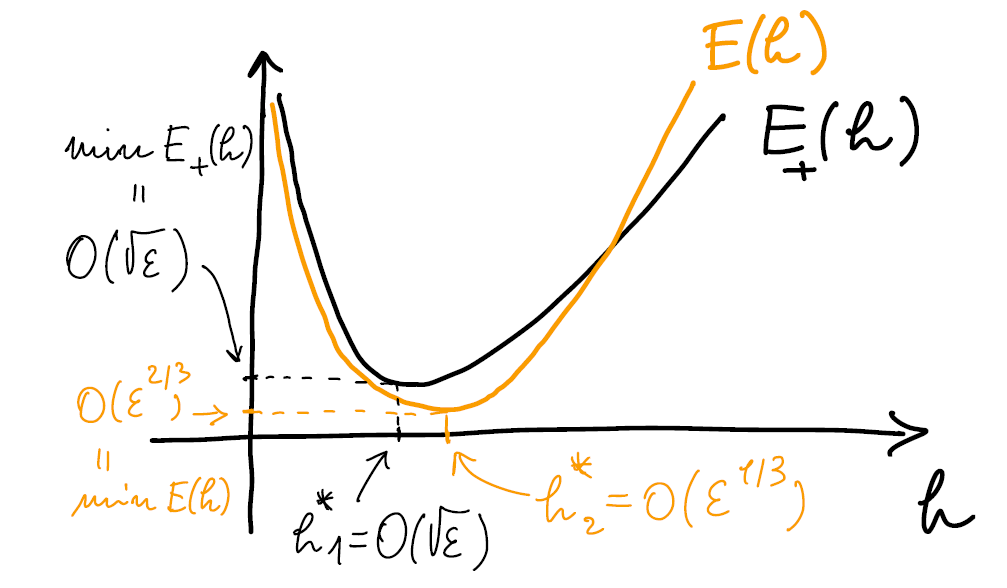
\includegraphics[width=0.6\textwidth]{pag29.png}
\end{center}
Questa analisi ci lancia un messaggio, parzialmente qualitativo ma chiaro: nel calcolo approssimato
%PAGINA 30 \\ % michele
della derivata non conviene campionare con un passo troppo piccolo, perché questo potrebbe amplificare in modo inaccettabile l'errore di misura/calcolo.\\
Per evitare di usare passi troppo piccoli convengono formule di approssimazione della derivata del tipo
\[
\phi(h) = f'(x) + \mathcal{O}(h^p)
\]
con $p$ possibilmente grande.\\
Vedremo nella prossima lezione che esiste un metodo generale se $f$ è regolare (il metodo di
%PAGINA 31 \\ % michele
"estrapolazione") per aumentare $p$ con un basso costo computazionale.\\
Per concludere osserviamo che abbiamo analizzato formule per il calcolo \underline{puntuale} della derivata tramite rapporti incrementali.\\
Sappiamo però che esistono metodi per l'approssimazione \underline{globale} della derivata (non in un singolo punto ma su tutto un intervallo) ad esempio l'interpolazione \underline{spline}.\\
Infatti se $f \in C^4 [a,b]$, usando le spline cubiche $S_3$ si ha
%PAGINA 32 \\ % michele
\[
dist(f', S'_3) = \mathcal{O}(h^3)
\]
È bene però ribadire che anche questo approccio soffre del problema dell'instabilità, in particolare si può far vedere (non lo faremo) che se $\tilde{S}_3$ è la spline cubica costruita su valori
\[
\tilde{y}_i : \abs{\tilde{y}_i - f(x_i)} \le \varepsilon
\]
allora
\[
dist(S'_3, \tilde{S}'_3) = \mathcal{O}(\varepsilon/h)
\]
rientrando nella problematica già trattata (visto che $\varepsilon/h \to \infty$ per $\varepsilon$ fissato e $h \to 0$).\\
%PAGINA 33\\ %Andrea
\underline{Nota facoltativa}: la disuguaglianza appena scritta non è altro che una \underline{disuguaglianza triangolare} per la \underline{distanza} tra funzioni continue che stiamo utilizzando, cioè \\
\begin{center}
$dist(f,g) = \underset{x \in [a,b]}{max} |f(x)-g(x)|$\\
\end{center}
Infatti $\forall f,g,\phi \in C[a,b]$ vale \\
\begin{center}
$dist(f,\phi)\leq dist(f,g) + dist(g,\phi)$\\
\end{center}
\underline{Dimostrazione}:\\
Fissato $x\in [a,b]$, per la disuguaglianza triangolare in $\mathbb{R}$
\[
| f(x) - \phi(x) | = | f(x) - g(x) + g(x) - \phi(x) | \leq | f(x) - g(x) | + | g(x) - \phi(x) |
\]
%PAGINA 34%Andrea 
Prendendo il max per $x \in [a,b]$ ad ambo i membri si ottiene
\[ \begin{split}
\underset{x \in [a,b]}{\max} |f(x)-g(x)| & \leq \underset{x \in [a,b]}{\max} \{ |f(x)-g(x)| + |g(x)-\phi(x)| \} \\
& \leq \underset{x \in [a,b]}{\max} |f(x)-g(x)|+ \underset{x \in [a,b]}{\max} |g(x)-\phi(x)|
\end{split} \]
dove abbiamo usato il fatto che date $u,v \in C[a,b]$
\[
\max\Big( u(x)+v(x) \Big) \leq \max \ u(x) + \max \ v(x)
\]

\end{document}
